\hypertarget{colorscheme}{There are three} ways to make a new color scheme:
\begin{itemize}
\item[--]with the command \pgfPTMmacro{pgfPTnewColorScheme}[]
\item[--]using the \textit{script} in the file \mbox{\href{run:pgfPTcolorSchemes.html}{pgfPTcolorSchemes.html}}
\item[--]with the commands provided by the \hyperlink{lib:colorschemes}{colorschemes library} (see the \hyperlink{sec:lib}{libraries section}).
\end{itemize}\ %
\\ [-44pt]\ %
\def\tmpSection{\textcolor{blue!50!black}{\textbackslash pgfPTnewColorScheme}}%
\subsection*{}{{\normalfont\large\bfseries\raisebox{1.25pt}{$\maltese$\ Designing a color scheme with \tmpSection}}%
\label{design:CSscheme}\addcontentsline{toc}{subsection}{\texorpdfstring{$\maltese$\ Designing a color scheme with \tmpSection}{\textbackslash pgfPTnewColorScheme}}%
\\ [4pt]This command provides a way to set the cell background color of each of the 118 elements of the Periodic Table. \textit{If the intention is to set the background color for all of them, it is highly recommended to use the file pgfPTcolorSchemes.html}, unless the trailing color begin at a small atomic number.
\\ [4pt]Despite that, this command can always be used taking into account:
\begin{enumerate}
\item It has the form \pgfPTMmacro{pgfPTnewColorScheme}[trailing color]\blue{\{}\red{name}\blue{\}\{}\red{color list}\blue{\}} where:
\begin{itemize}
\item[--] the first argument (enclosed by square brackets) is optional. If provided, the specified trailing color will be used, otherwise the default color (white) will be used as trailing color.%The trailing color will be used after the last color given in the color list.
\item[--] the second and third arguments are mandatory and specify, respectively, the color scheme name and the color list.
\end{itemize}
\item The \red{name} is any name made up of letters (only the characters a,\myldots,z and A,\myldots,Z).
\item The \red{color list} is a comma-separated list where each entry has the format \red{r/g/b}, representing the red, blue and green values, between 0 and 1, of the color: the first entry of the list will be the background color used in the cell of the element with atomic number 1, the second entry, the background color of the cell of the element with atomic number 2, and so on.
\\ [8pt]\tikz{\node[text width=\linewidth-.6666em,fill=green!5!white,draw=green!50!black,rounded corners=2pt] {%
\textit{If the color list has ten entries, these entries will set the background colors of the elements with atomic numbers from 1 to 10.  For the following atomic numbers, greater than or equal to 11, the \red{trailing color} will be used in the color background}.
};}
\end{enumerate}
\ %
\\ [-44pt]\ %
\def\tmpSection{\textcolor{cyan}{pgfPTcolorSchemes.html}}%
\subsection*{}{{\normalfont\large\bfseries\raisebox{1.25pt}{$\maltese$\ Designing a color scheme with \tmpSection}}%
\label{design:CSscheme}\addcontentsline{toc}{subsection}{\texorpdfstring{$\maltese$\ Designing a color scheme with \tmpSection}{pgfPTcolorSchemes.html}}%
\vfill\makebox[\linewidth][c]{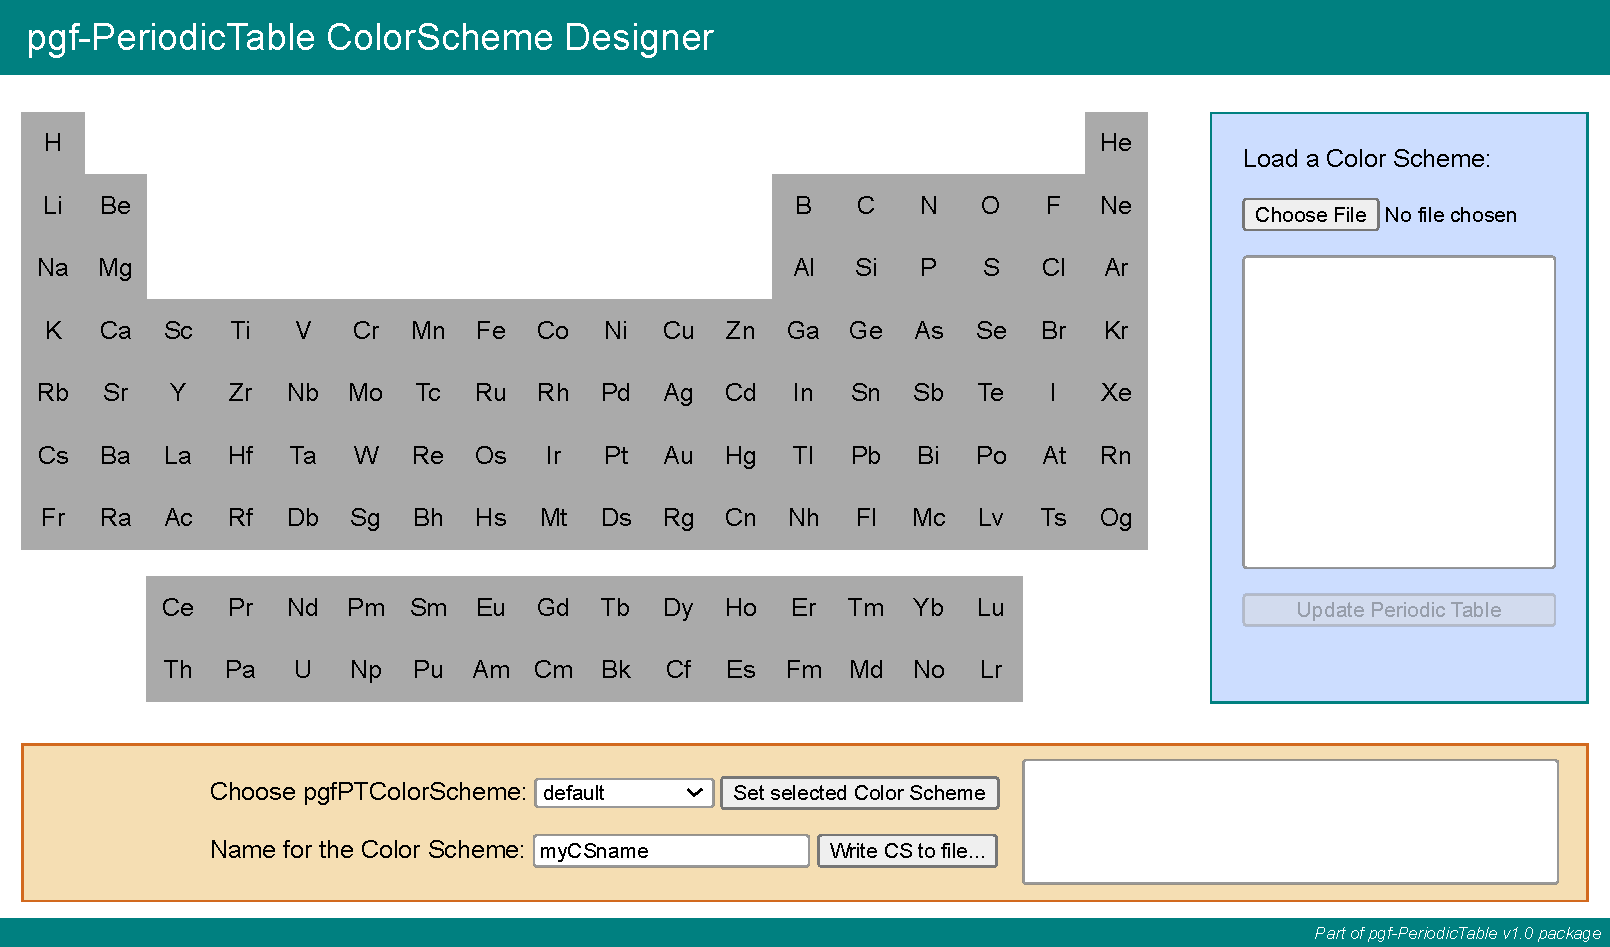
\includegraphics[width=.5\linewidth]{manualfiles/pgfPTcolorSchemes_html_general.pdf}}
\vfill The \href{run:pgfPTcolorSchemes.html}{pgfPTcolorSchemes.html} \textit{designer} is an \textit{html} file with a little \textit{javascript} code to perform the task of building a color scheme to use with the \red{back color scheme} key associated with the \blue{\textbackslash pgfPT} command.
\newpage The Periodic Table of the Elements is displayed on the page and clicking on an element opens a color dialog:
\\ [4pt]\makebox[\linewidth][c]{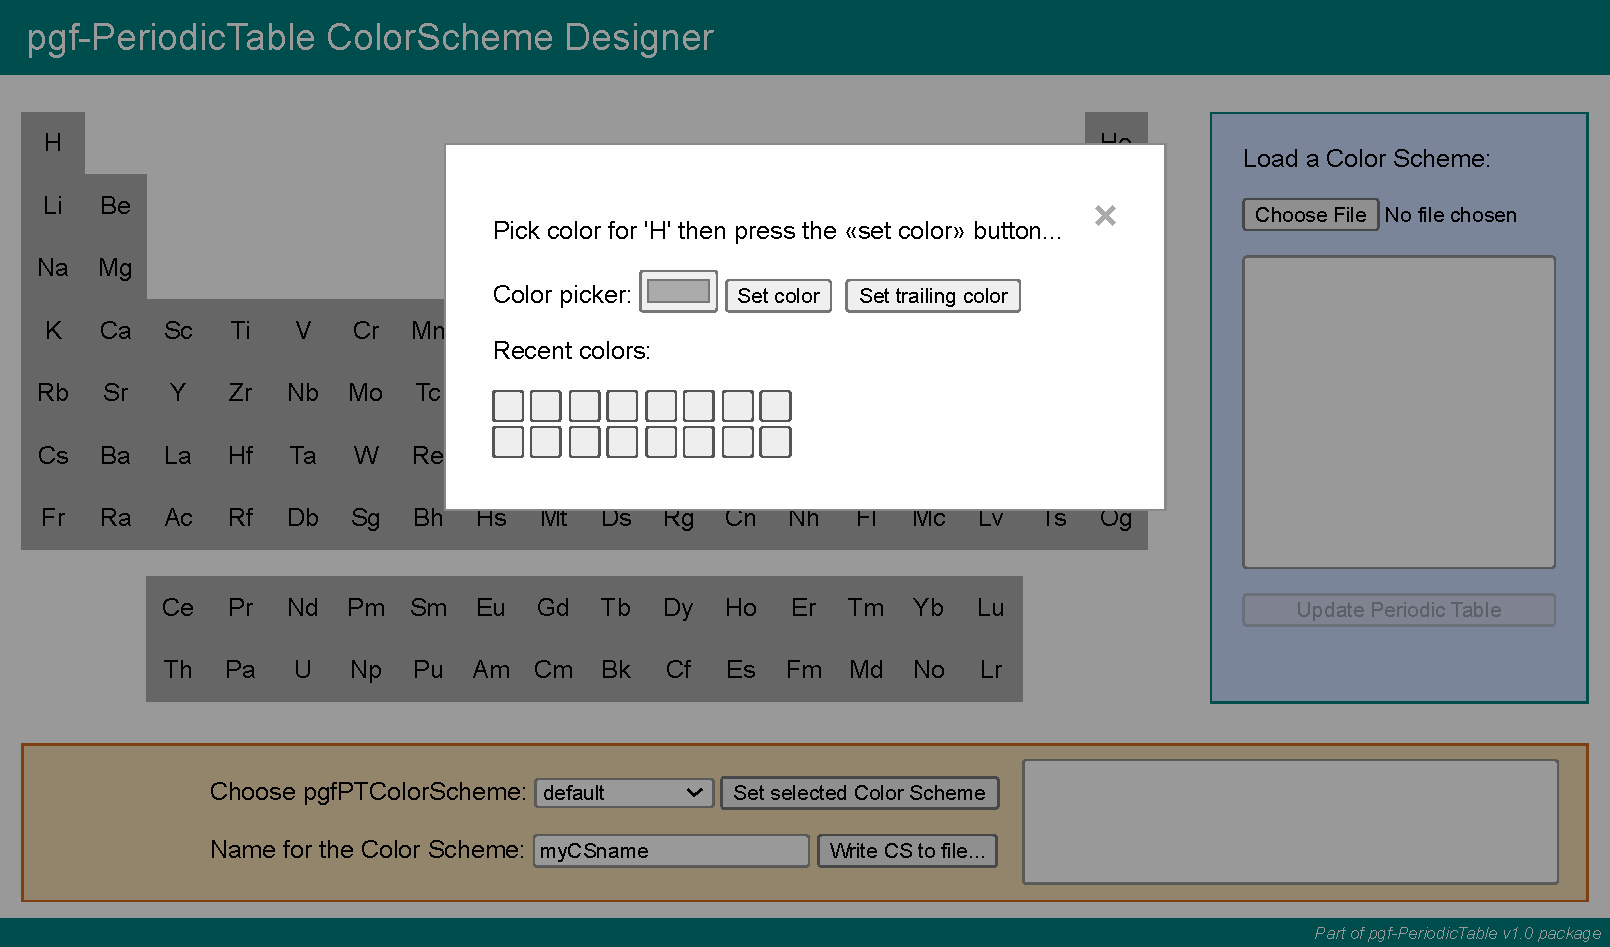
\includegraphics[width=.7\linewidth]{manualfiles/pgfPTcolorSchemes_html_color.pdf}}
\setbox0=\hbox{\tikz{\draw[btnBorder,fill=black!67] (0,0) rectangle (7.5mm,3mm);}}%
\\ [8pt]Clicking on the {\small Color picker:\hspace{.2ex}}\pgfPTMbtn{\usebox0} button opens a color dialog, where there is the possibility to choose the desired color or manually enter one color using one of the three models available (RGB, HSL or HEX):
\\ [4pt]\makebox[\linewidth][c]{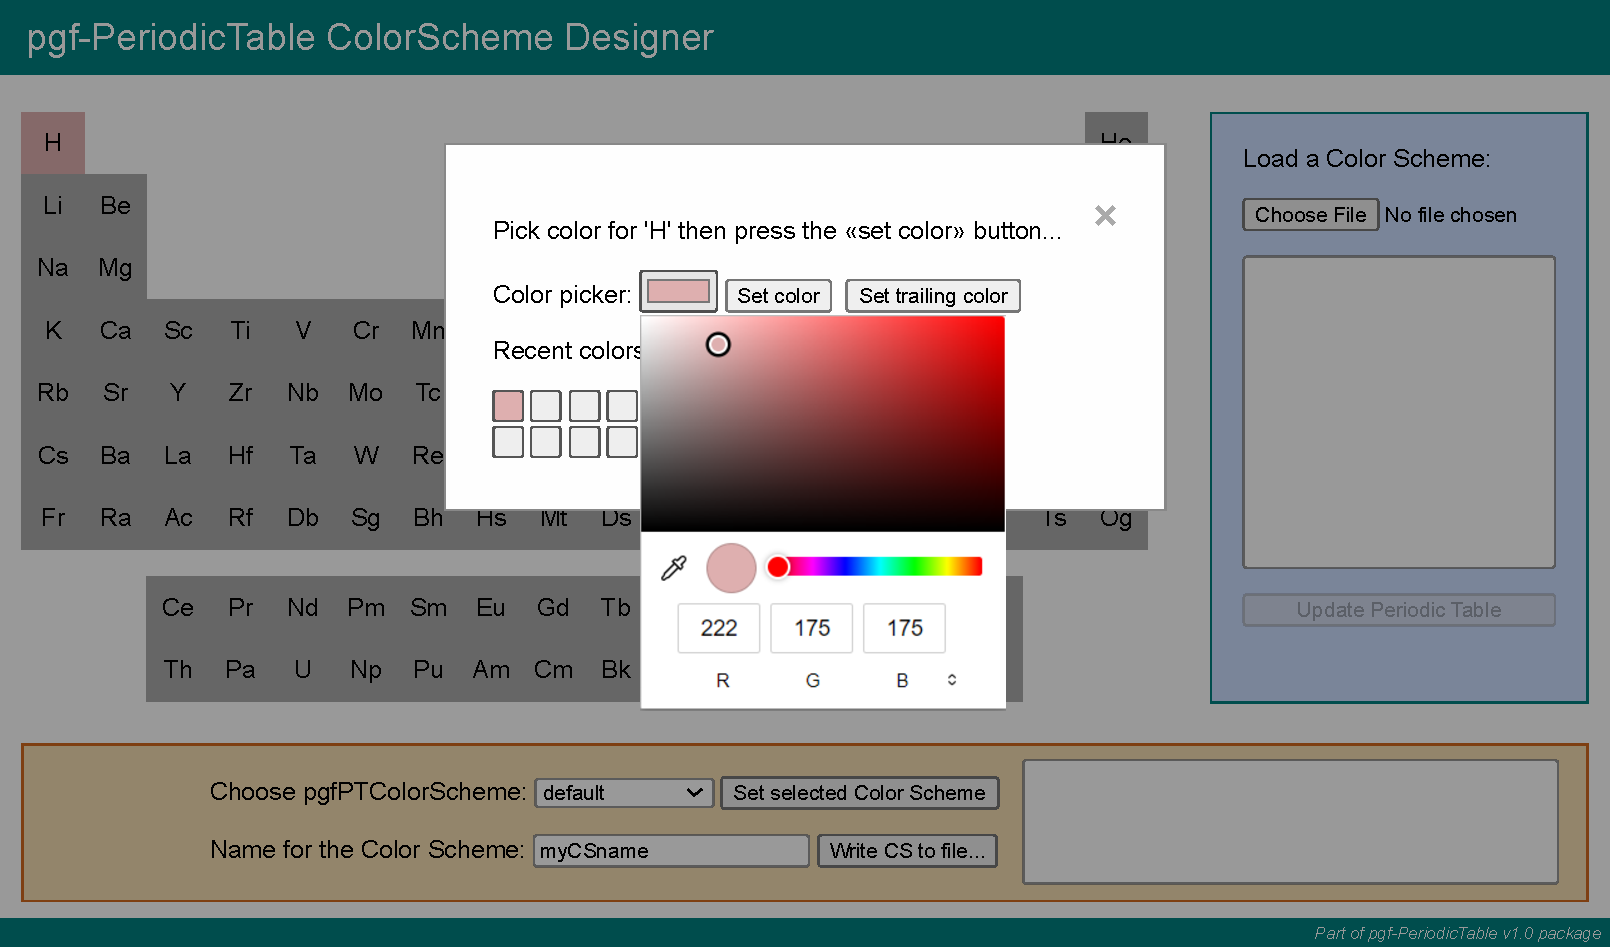
\includegraphics[width=.7\linewidth]{manualfiles/pgfPTcolorSchemes_html_colorPicker.pdf}}
\\ [8pt]After changing the desired colors it is possible to save the color scheme in a file by clicking on \pgfPTMbtn{Write CS to file...}:
\\ [4pt]\makebox[\linewidth][c]{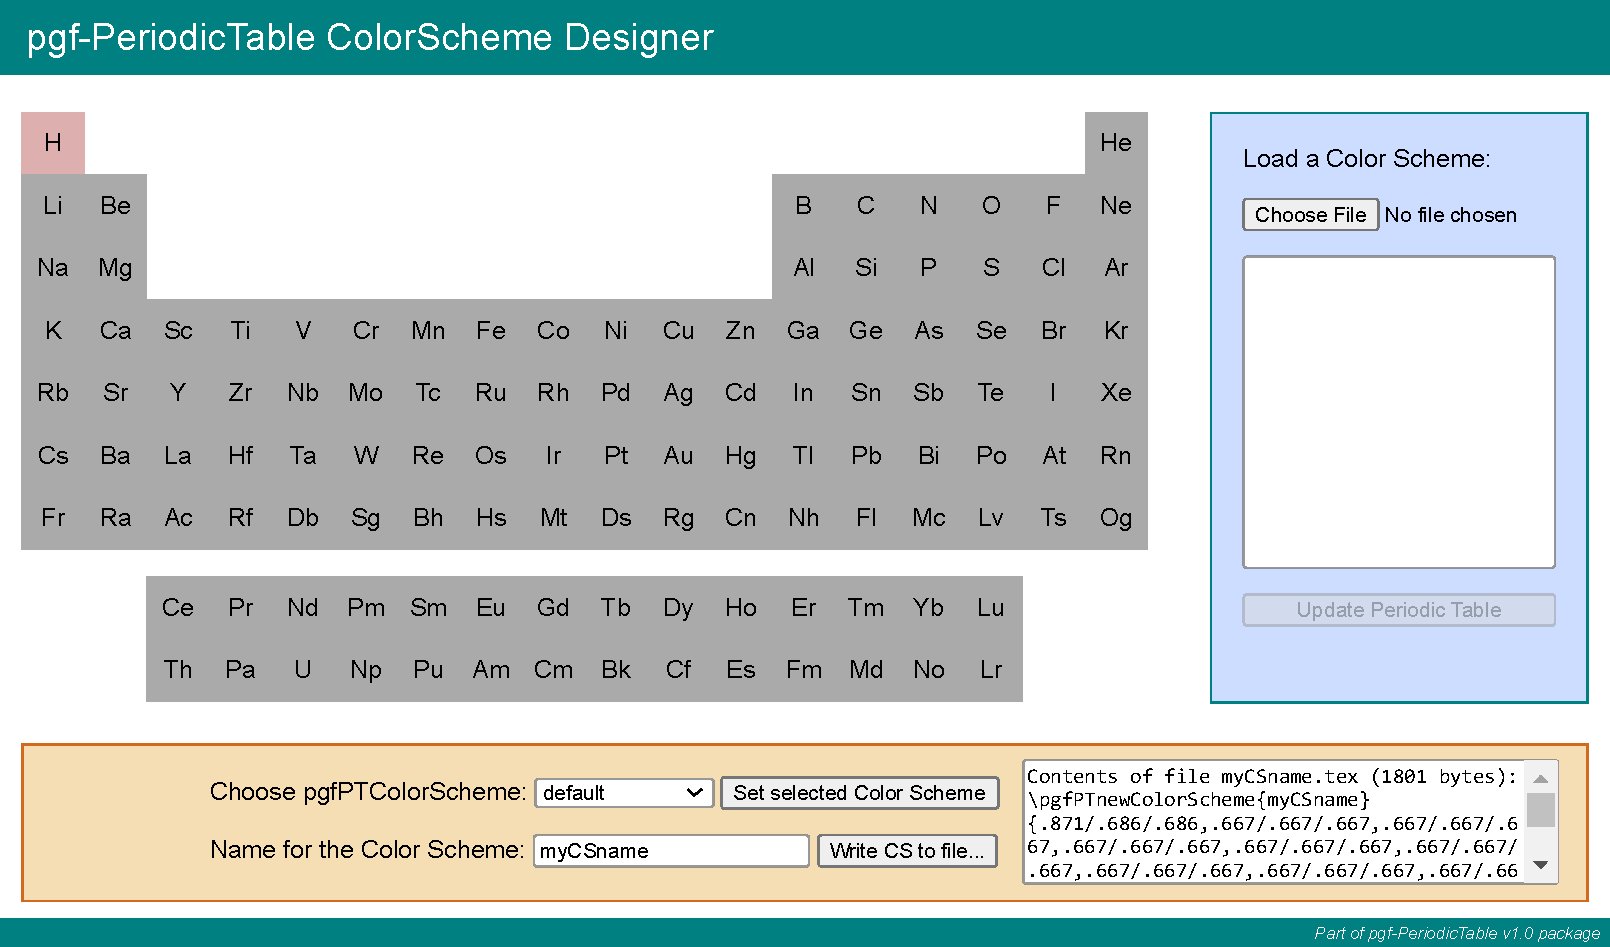
\includegraphics[width=.7\linewidth]{manualfiles/pgfPTcolorSchemes_html_save.pdf}}
\\ [8pt]To use a color scheme saved in a file there are two possible ways:
\begin{itemize}
\item[--]loading the file in the working document via the {\large\textsf{\textbackslash input}} \LaTeX{} command, for instance, {\large\textsf{\textbackslash input\{myCSname.tex\}}}.
\item[--]or by opening the file and copying and pasting its contents into the working document.
\end{itemize}
In either case, the operation can be performed at any location in the document, but before the named color scheme is used.
\\ [4pt]Note that in the previous example there is only one color that has been defined (for hydrogen). In that case, it is useful to set the trailing color in helium by clicking in \pgfPTMbtn{Set trailing color} (which automatically changes to \pgfPTMbtn{Remove trailing color}). After that only the hydrogen and helium are clickable, all the other elements are locked to click:
\\ [4pt]\makebox[\linewidth][c]{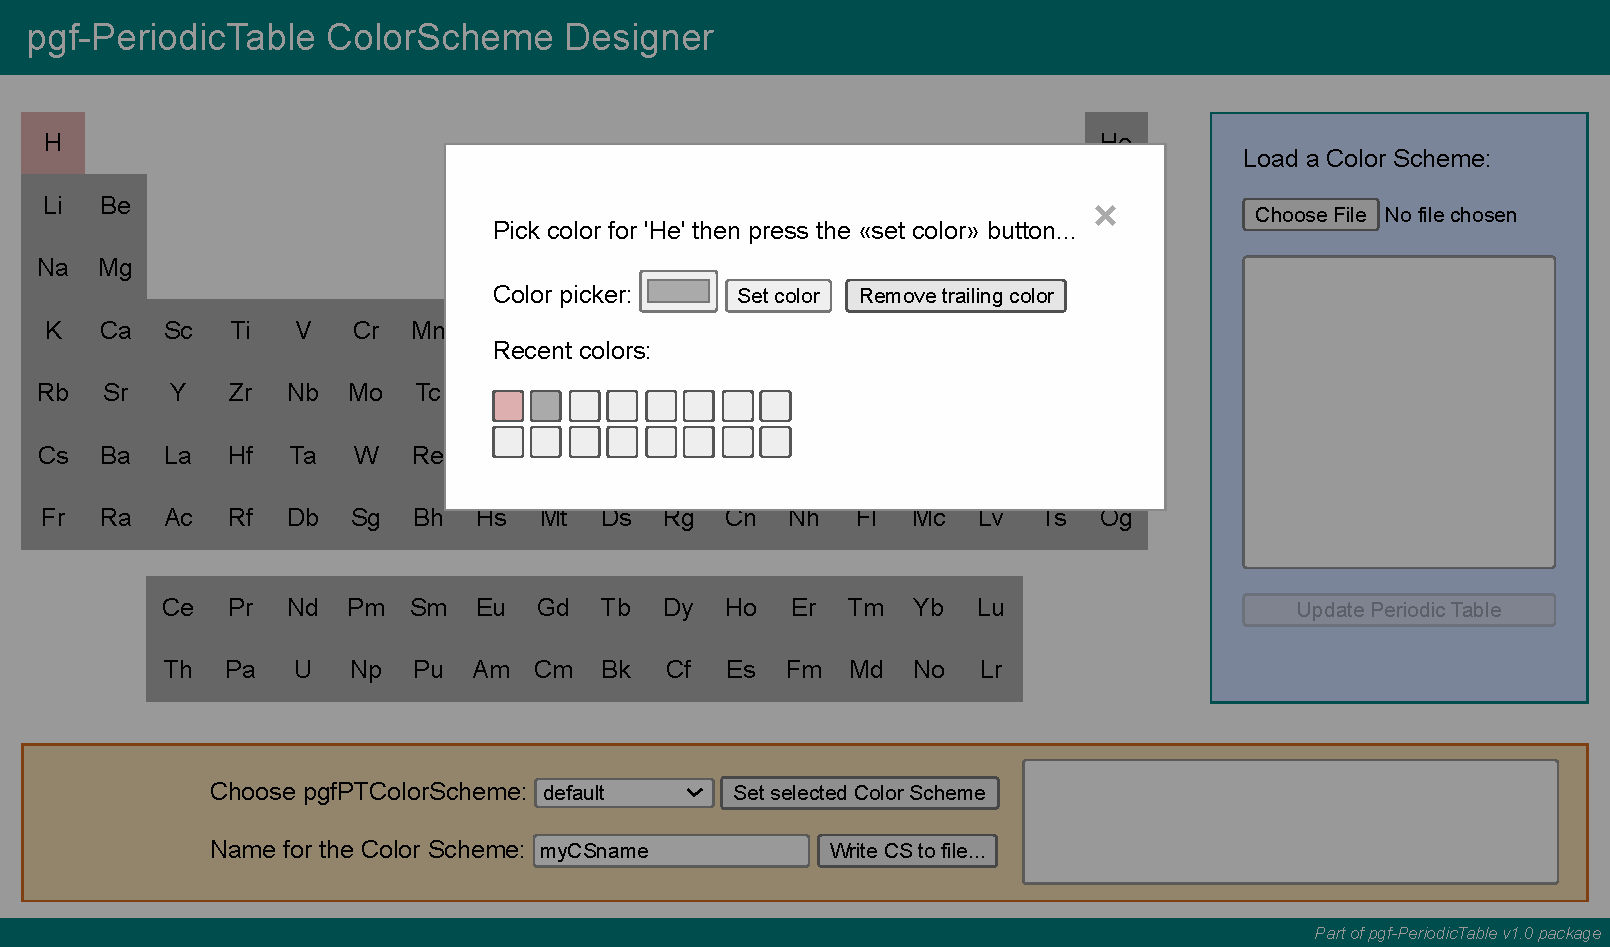
\includegraphics[width=.7\linewidth]{manualfiles/pgfPTcolorSchemes_html_trailing.pdf}}
\\ [8pt]Then the saved color scheme will have the optional trailing color and the size will be smaller as only the color codes of the changed elements are stored:
\\ [4pt]\makebox[\linewidth][c]{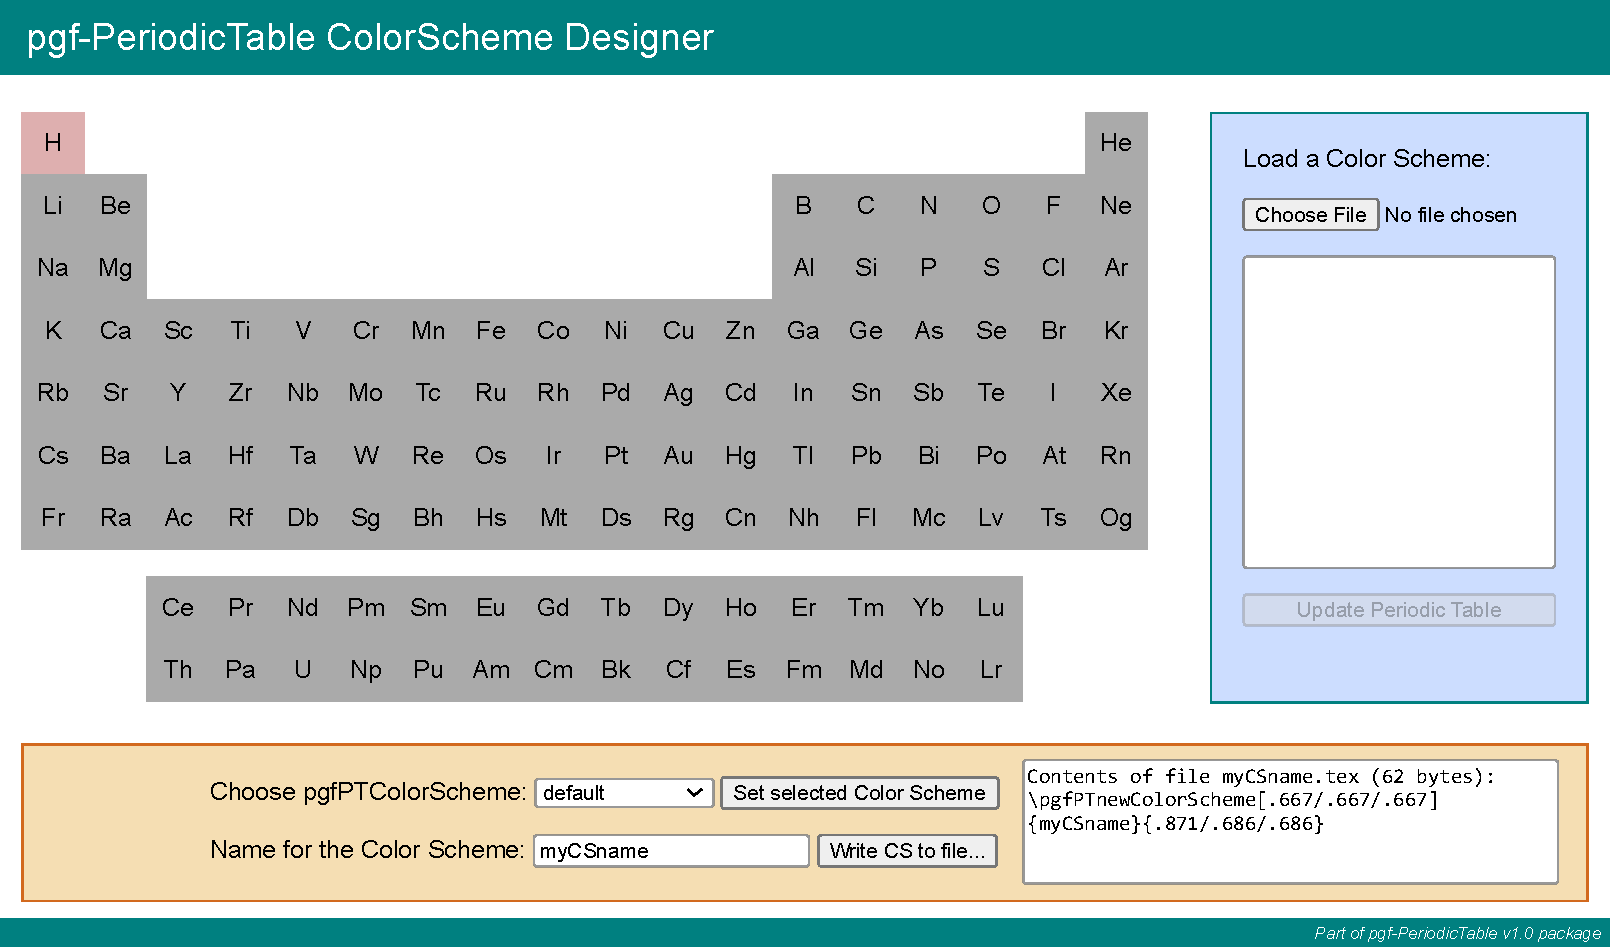
\includegraphics[width=.7\linewidth]{manualfiles/pgfPTcolorSchemes_html_saveTrailing.pdf}}
\\ [8pt]To remove the trailing color click on the last enabled element (in the  above case helium) and then click on \pgfPTMbtn{Remove trailing color}. After that, all elements can be clicked again.
\\ [8pt]It is also possible to load a color scheme saved to a file by clicking on \pgfPTMbtn{Choose File} and then clicking on \pgfPTMbtn{Update Periodic Table} for the color scheme to take effect:
\\ [4pt]\makebox[\linewidth][c]{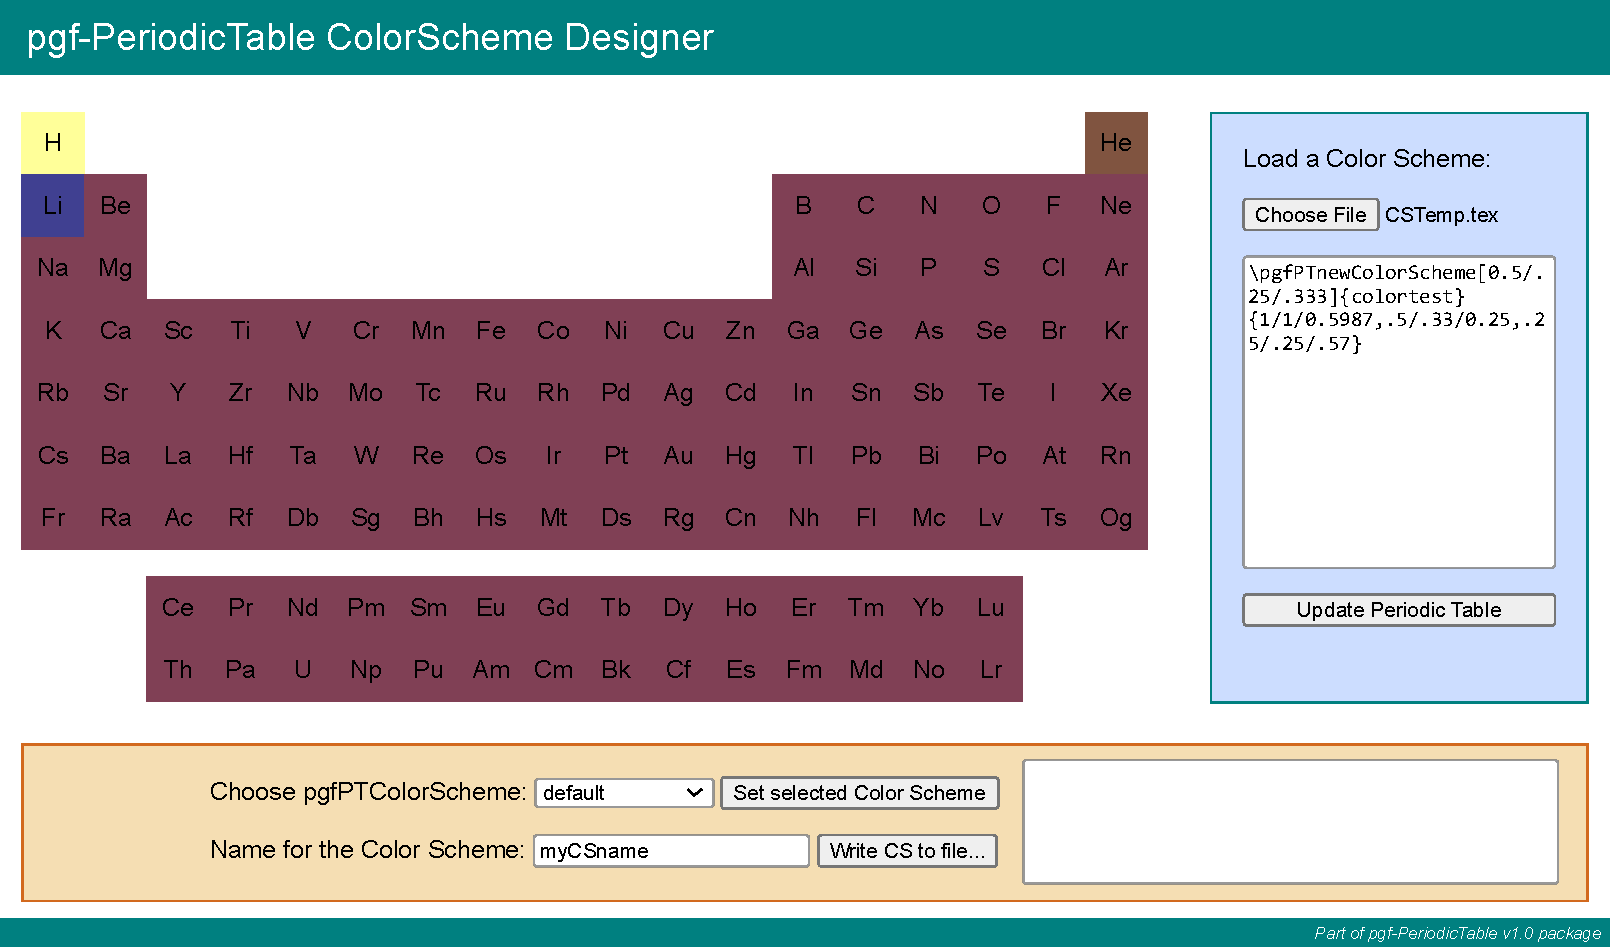
\includegraphics[width=.7\linewidth]{manualfiles/pgfPTcolorSchemes_html_load.pdf}}
\\ [4pt]Finally its possible to load a built-in color scheme by choosing a named \textit{pgfPTColorScheme} in the corresponding combo box and then clicking on \pgfPTMbtn{Set selected Color Scheme}:
\\ [4pt]\makebox[\linewidth][c]{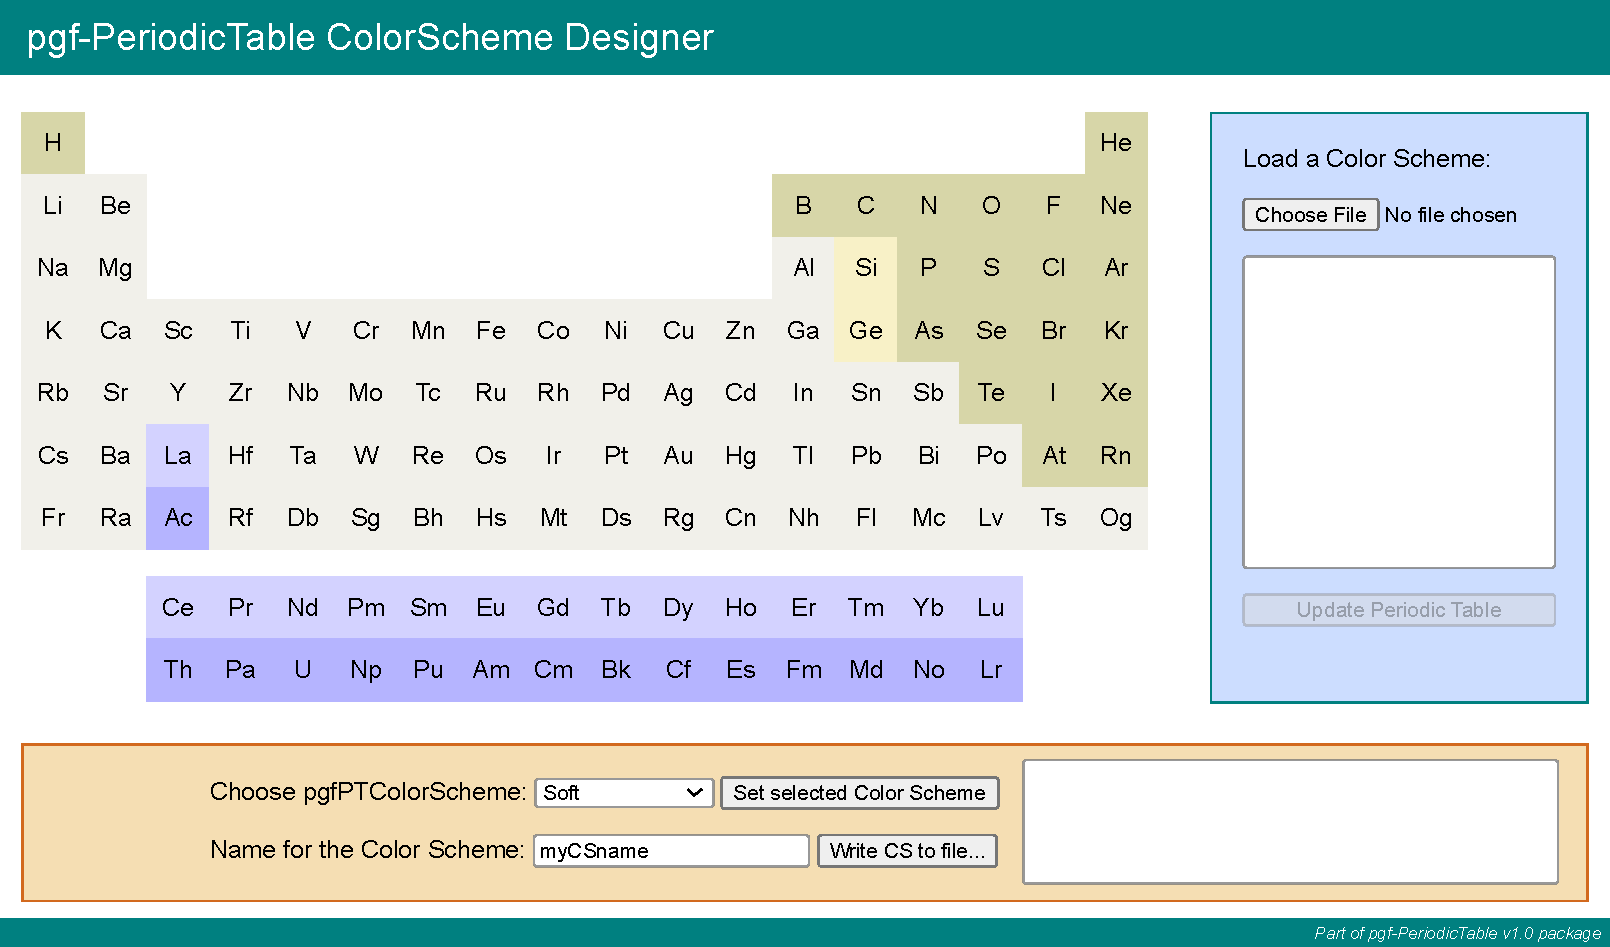
\includegraphics[width=.7\linewidth]{manualfiles/pgfPTcolorSchemes_html_set.pdf}}
\\ [20pt]\makebox[\linewidth][c]{\textit{All the operations described are always available}.}
\endinput
